% team-meeting-2026-11-18-slides.tex -- open questions and a proposed plan for the one
% final summary pass over the production scenario output, team meeting of November 18,
% 2026 (30 minutes). Turns the email sent on 2026-11-16
% (docs/meetings/summary-tables-email-sent-2026-11-16.org) into decisions.
% Build: plain pdflatex (emacs, emacs-r container) or xelatex (bittensor-ubuntu), run
% twice. beamerthemeozlabs.sty, ozcolors.sty and ozfonts.sty in this directory are
% symlinks to ~/code/oz-templates/, and the logo is set by absolute path below, so no
% TEXINPUTS setting is needed.
% Numbers: the range example is from the 2026-11-06 pooling, rebuilt with the WBG groups
% (review/multimodel-2026-11-wbg/tables/world_and_income_groups_totals.csv); the
% summing and independence ranges are from docs/meetings/summary-tables-request-2026-11-16.org.
% Backup figures are copied from review/multimodel-2026-11-wbg/figures-slides/.
\documentclass[aspectratio=169,11pt]{beamer}

\usetheme{ozlabs}

\renewcommand{\ozfootbrand}{OZ Labs}
\renewcommand{\ozfooturl}{ozlabs.tech}
\renewcommand{\ozeyelogo}{/var/home/aoz/code/oz-templates/assets/ozlabs-seed-logo.pdf}

\usepackage{booktabs}
\usepackage{array}
\newcolumntype{L}[1]{>{\raggedright\arraybackslash}p{#1}}

\title{One Final Summary Pass: Open Questions and a Plan}
\subtitle{What to compute from the scenario output before the per-draw files are deleted}
\author{Aaron Osgood-Zimmerman}
\institute{OZ Labs, for the World Bank}
\date{November 18, 2026}

\begin{document}

\begin{frame}[plain,noframenumbering]
  \titlepage
\end{frame}

\begin{frame}{What I'd like us to decide today}
  \small
  Follow-up to my email of November 16. I'd like to leave with an answer to each of these, or a name and a date for one:
  \begin{enumerate}
    \item \textbf{Anything missing from the table list?} Places, periods, breakdowns, measures or statistics.
    \item \textbf{Periods:} decades only, or also single years, or 5-year periods?
    \item \textbf{Age standard} for age-standardized rates: GBD world standard or WHO 2000--2025?
    \item \textbf{Valuation:} is the valuation math already fixed?
    \item \textbf{Keeping the output:} the full output, a compact copy, or tables only; and who stores it?
    \item \textbf{Historical sources:} the two GBD rounds as planned, and do we want a 2000 value?
    \item \textbf{Showing historical data:} which round, which measure, which figures, and where?
  \end{enumerate}
  \medskip
  Then the plan: I write and test the code, Caspar runs it once, and I check it before anything is deleted.
\end{frame}

\begin{frame}{Why it has to be one pass, listed up front}
  \small
  Means can be added up later from summary tables. Uncertainty ranges can't: draw $d$ uses the same risk-curve and mortality-forecast draw in every country, year, cause and age, so cells move together.

  \medskip
  \centering
  \begin{tikzpicture}[x=0.0115cm,y=0.5cm,font=\footnotesize]
    % axis in thousands of deaths per year, 350 to 1150
    \draw[oztextsec] (350,0) -- (1150,0);
    \foreach \v in {400,600,800,1000} {
      \draw[oztextsec] (\v,0) -- (\v,-0.15) node[below,text=oztextsec] {\v};
    }
    \node[text=oztextsec,anchor=north] at (750,-0.75) {Heat deaths per year, thousands};
    % mean
    \draw[oztextmuted,dashed] (670,0.2) -- (670,3.8);
    \node[text=oztextsec,anchor=south] at (670,3.75) {mean 670};
    % correct
    \draw[ozcyan,line width=2.2pt] (456,3) -- (992,3);
    \node[anchor=east,text=oztext] at (440,3) {Correct (from the draws)};
    \node[anchor=west,text=oztextsec] at (1000,3) {456 to 992};
    % summed bounds
    \draw[ozmagenta,line width=2.2pt] (390,2) -- (1102,2);
    \node[anchor=east,text=oztext] at (380,2) {Adding country bounds};
    \node[anchor=west,text=oztextsec] at (1110,2) {390 to 1,102};
    % independent
    \draw[ozpurplelight,line width=2.2pt] (542,1) -- (798,1);
    \node[anchor=east,text=oztext] at (530,1) {Countries independent};
    \node[anchor=west,text=oztextsec] at (806,1) {542 to 798};
  \end{tikzpicture}

  \raggedright\footnotesize
  Low- and middle-income countries, heat deaths, SSP2-4.5, 2041--2050, 95\% ranges. Adding the countries' bounds overstates the range; treating countries as independent understates it. The same holds for any total we don't compute now, including valued (monetary) totals.
\end{frame}

\begin{frame}{The proposed tables (as in my email)}
  \scriptsize
  \renewcommand{\arraystretch}{0.95}
  \begin{tabular}{L{0.16\textwidth}L{0.78\textwidth}}
    \toprule
    Scenarios & SSP1-2.6, SSP2-4.5 (reference), SSP3-7.0, SSP5-8.5; pooled over the 24 common climate models $\times$ 500 draws \\
    Measures & Deaths and years of life lost (YLLs), each for heat, cold, and heat + cold \\
    Statistics & Mean, and 95\%, 80\%, 66\% ranges; for the three other scenarios also the difference from SSP2-4.5, draw by draw \\
    Context & Population and IHME's forecast deaths, for rates \\
    Places & 204 countries, world, 4 income groups, low and middle income combined, 7 World Bank regions \\
    Periods & 2022--2030, 2031--2040, 2041--2050, and 2022--2050 \quad \textcolor{ozmagenta}{\textbf{open: single years or 5-year periods too?}} \\
    Breakdowns & Totals; sex; age; age $\times$ sex; cause; cause $\times$ sex; cause $\times$ age; cause $\times$ age $\times$ sex \\
    Ages & 17 five-year groups (0--4 to 80+), plus under 5, 15--49, 15--64 (working age), 50--69, 65+ \\
    Causes & The 17 causes; cardiovascular (4 causes); diabetes and kidney disease; injuries (9 causes); all causes except forces of nature (for Haiti and Honduras) \\
    Age-standardized & Deaths and YLLs per 100,000, heat, cold, heat + cold; every place and period; by sex and by cause group; \textcolor{ozmagenta}{\textbf{open: which standard to report}} \\
    \bottomrule
  \end{tabular}

  \medskip
  \raggedright
  \textbf{Question 1: anything missing?} Anything not listed gets correct means later from the tables, but a valid range only from a new summary run over the draws, which needs the draws kept (Question 5). (Crude rates are fine: population is fixed, so their ranges follow from the count tables.)
\end{frame}

\begin{frame}{Question 2: which periods?}
  \small
  \begin{tabular}{L{0.25\textwidth}L{0.33\textwidth}L{0.30\textwidth}}
    \toprule
    Option & What it allows & Largest table \\
    \midrule
    Decades and 2022--2050 only & Everything in the current report & About 2 GB of text \\
    Plus single years & Yearly series with ranges; the inputs to a discounted valuation (means only) & About 13 GB of text \\
    Plus 5-year periods & 5-year totals with ranges & Small addition \\
    \bottomrule
  \end{tabular}

  \medskip
  \raggedright\footnotesize
  \begin{itemize}
    \item Sizes are my arithmetic for the table split by country, year, age, sex and cause, not measured. Size isn't a constraint either way.
    \item A range on a 5-year or decade total can't be built from yearly ranges, so each period we want ranges for has to be listed now or summarized again from the draws.
    \item \textbf{My suggestion:} add single years, since a valuation with discounting is done year by year, and add 5-year periods only if someone needs them. Cheap to include now; adding it later means another summary run over the draws, possible only if we keep them.
  \end{itemize}
\end{frame}

\begin{frame}{Question 3: which age standard?}
  \small
  \begin{itemize}
    \item The pass computes age-standardized rates under both standards, so this decides only which one we report; it doesn't hold up the run.
    \item GBD world standard population: the one GBD uses, so our rates line up with GBD's published rates, including the historical comparison.
    \item WHO 2000--2025 standard: WHO's own standard population.
    \item Both have finer groups above 80; I sum them into 80+ to match our age groups.
    \item \textbf{My suggestion:} report the GBD world standard, since our method and our comparisons are GBD's, and put the other in an appendix table. Charlie's vote at the last meeting was for age-standardized rates for comparability; I'd defer to the team on which standard the World Bank's audience expects.
  \end{itemize}
\end{frame}

\begin{frame}{Question 4: valuation}
  \large
  \medskip
  \textbf{Is the valuation math already fixed?}

  \bigskip\normalsize
  \begin{itemize}
    \item If yes, valued totals with ranges can go in this pass.
    \item If no, a valid range on a valued total later needs the draws (Question 5).
  \end{itemize}
\end{frame}

\begin{frame}{Question 5: what do we keep, and who stores it?}
  \scriptsize
  \centering
  \renewcommand{\arraystretch}{0.95}
  \begin{tabular}{L{0.20\textwidth}L{0.12\textwidth}L{0.29\textwidth}L{0.27\textwidth}}
    \toprule
    Option & Size & What it allows later & Cost and risk \\
    \midrule
    (a) Full scenario output as it is & Roughly 10 TB & Any new total with a valid range & Hard to host \\
    \midrule
    (b) Compact copy, written in the same pass & Roughly 50 to 70 GB & The same as (a): the full output rebuilds exactly from it, with scripts I'd supply & Exact rebuild checked on only 4 local Colombia files; the pass checks a sample of production files before anything is deleted \\
    \midrule
    (c) Tables only & The tables (Question 2) & Only what's in the tables; new totals get means, no ranges & Nothing to host \\
    \bottomrule
  \end{tabular}

  \medskip
  \raggedright\footnotesize
  \begin{itemize}
    \item Sizes: 10 TB scales Caspar's benchmark of about 52 GB per country; 50 to 70 GB is my arithmetic. Neither is measured.
    \item Compact copy: attributable fractions and scale factors per draw, plus IHME deaths per draw and population; attributable deaths are their product.
    \item \textbf{My suggestion:} (b). \textbf{For Charlie and Caspar:} where can 50 to 70 GB live, and who looks after it? Caspar shouldn't delete anything until this is settled and the rebuild check has passed.
  \end{itemize}
\end{frame}

\begin{frame}{Question 6: historical sources}
  \small
  \begin{itemize}
    \item No new runs: GBD's published estimates, already on disk.
    \begin{itemize}\small
      \item GBD 2019 round (Burkart et al.\ 2021 companion data): 1990, 2010, 2019. This is the round our method follows; our 2022 total was 1.07 times its 2019 estimate, with 182 of 204 countries inside its 95\% range.
      \item GBD 2023 round: 2019 and 2022. GBD revised heat upward between rounds, mostly in hot countries, so its heat numbers are higher than ours (our 2022 heat is 0.68 to 0.77 times its value).
    \end{itemize}
    \item I've put these next to our results as crude rates per 100,000 (the 2019-round file gives rates and percentages, not counts). Examples on the next three slides; how to show them is Question 7.
    \item A 2000 value exists only in the GBD 2023 round, so it would sit on the higher heat line. \textbf{My suggestion:} skip 2000 unless someone needs it.
  \end{itemize}
\end{frame}

\begin{frame}{Example: the world over time}
  \centering
  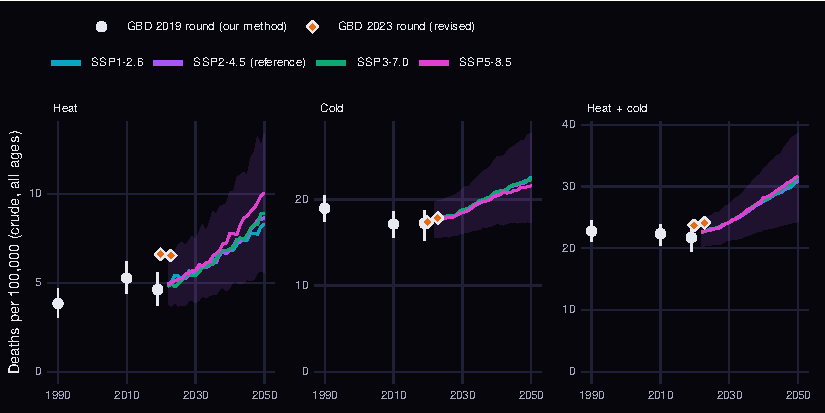
\includegraphics[width=\textwidth,height=0.64\textheight,keepaspectratio]{figures-2026-11-18/fig_hist_world.pdf}

  \footnotesize\raggedright
  Crude deaths per 100,000. Our 2022 (SSP2-4.5: heat 4.97, cold 17.65) is close to the GBD 2019 round's 2019 (4.62, 17.23), the round we follow; heat is below the revised 2023 round (6.54 in 2022). Crude rates rise partly because populations age.
\end{frame}

\begin{frame}{Example: income groups and the world}
  \centering
  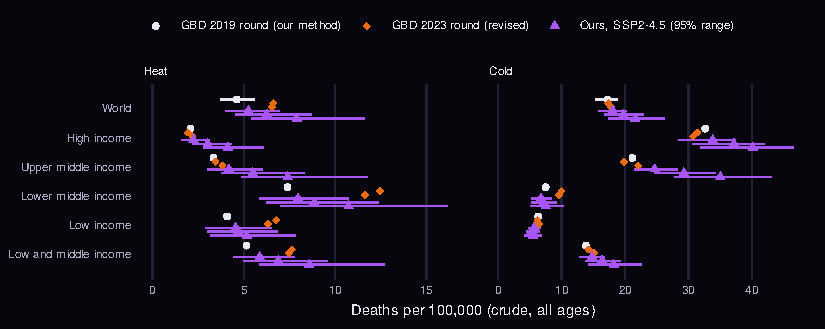
\includegraphics[width=\textwidth,height=0.59\textheight,keepaspectratio]{figures-2026-11-18/fig_hist_income.pdf}

  \footnotesize\raggedright
  Top to bottom in each group: GBD 2019 round (2019), GBD 2023 round (2019, 2022), our three decades (SSP2-4.5, 95\% ranges). GBD group values are sums over countries, so no range. The round revision is mostly heat in lower middle income (7.40 to 12.47 for 2019); ours follows the 2019 round (7.97 in 2022--2030).
\end{frame}

\begin{frame}{Example: four countries over time}
  \centering
  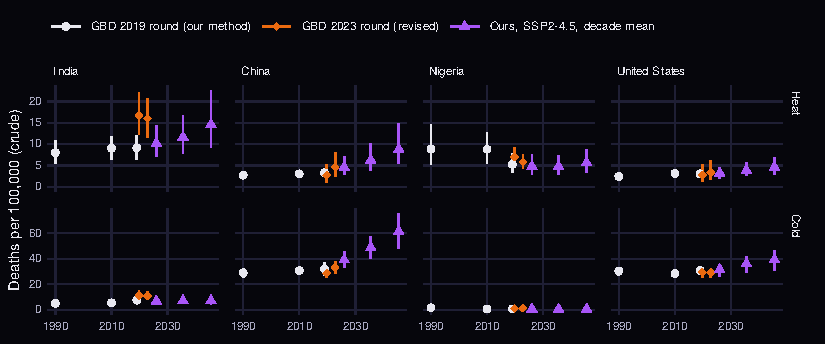
\includegraphics[width=\textwidth,height=0.64\textheight,keepaspectratio]{figures-2026-11-18/fig_hist_country_examples.pdf}

  \footnotesize\raggedright
  Our decade means (SSP2-4.5) are plotted mid-decade; all points with 95\% ranges. India shows the round revision most (heat 9.1 against 16.7 for 2019). China's cold rises in our projection; with crude rates I suspect much of that is aging (not yet split).
\end{frame}

\begin{frame}{Question 7: how do we want to show historical data?}
  \scriptsize
  \renewcommand{\arraystretch}{0.92}
  \begin{tabular}{L{0.12\textwidth}L{0.48\textwidth}L{0.30\textwidth}}
    \toprule
    Choice & Options & My suggestion \\
    \midrule
    Which GBD round & (a) 2019 round only, which matches our method; (b) both, the 2023 round labeled as revised; (c) 2023 round only, where our heat would look like a drop & (b): the 2019 round as the anchor, the revision visible \\
    \midrule
    Measure & Crude rates (now); age-standardized (ours after the final pass; the 2023 round needs another download); counts (2023 round only) & Age-standardized to compare, crude for the size of the burden \\
    \midrule
    Figures & World over time (earlier slide); groups side by side; a few countries over time; every country (table or scatter) & World and income groups in the main text; countries in an appendix \\
    \midrule
    Years & 1990, 2010, 2019 (2019 round); 2019, 2022 (2023 round); 2000 only from the 2023 round & As listed, no 2000 \\
    \midrule
    Groups & GBD's regions, or World Bank groups built from countries (no GBD range) & World Bank groups, to match the rest of the report \\
    \bottomrule
  \end{tabular}

  \smallskip\footnotesize\raggedright
  Is the comparison for context in the report, a check for us, or both? That decides how much goes in the main text.
\end{frame}

\begin{frame}{Also in the pass: numbers for our own checks}
  \small
  At countries, groups and world, by decade only, no age, sex or cause split:
  \begin{itemize}
    \item lowest and highest climate-model mean, and how many of the 24 models are above SSP2-4.5;
    \item the share of the range that comes from disagreement between climate models;
    \item attributable fraction (attributable deaths $\div$ IHME deaths), with ranges;
    \item the year heat overtakes cold: share of model-draw pairs crossing before 2022, in 2022--2050, and after 2050;
    \item population-weighted mean temperature per country, year, scenario and model.
  \end{itemize}
  \medskip
  These are for vetting, not for publication. \textbf{Does anyone want any of them at a finer level?}
\end{frame}

\begin{frame}{Proposed plan}
  \small
  \begin{enumerate}
    \item \textbf{Today:} settle the seven questions, or name who answers each and by when.
    \item \textbf{Aaron:} write the code for the pass from the settled list, and test it on a small test tree built from real Colombia output. It writes the tables, the compact copy if we choose it, and the rebuild check.
    \item \textbf{Aaron:} send Caspar the code and instructions, with output size and run time per file measured on the test tree.
    \item \textbf{Caspar:} one pass over the existing output, no model reruns. The last full read took about 153 CPU-hours, about 10 hours on 16 workers; this pass adds pooling and ranges on top, not yet measured.
    \item \textbf{Aaron:} check the tables and the rebuild check. Only then does anything get deleted.
    \item \textbf{Aaron:} revise the report and the slides with the final tables, the new groups and regions, and the historical comparison.
  \end{enumerate}
  \smallskip
  I'll start the code now from the current list, kept data-driven so additions are cheap.
\end{frame}

\appendix

\begin{frame}{Backup: World Bank regions, crude rates}
  \centering
  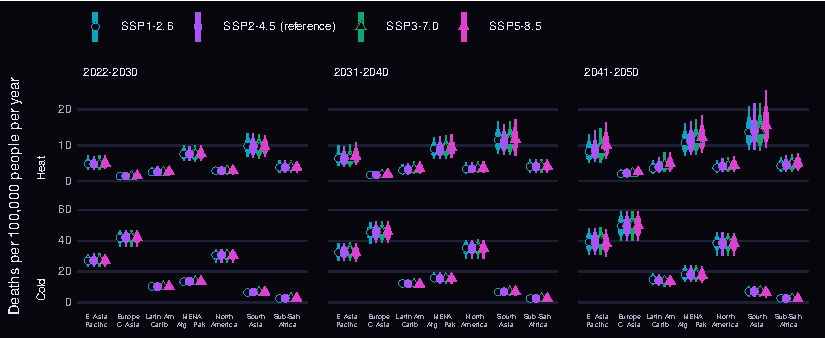
\includegraphics[width=0.9\textwidth,height=0.72\textheight,keepaspectratio]{figures-2026-11-18/fig_region_rates.pdf}

  \footnotesize\raggedright
  New since November 9: the seven World Bank regions from the official classification file. Crude rates, not age-standardized.
\end{frame}

\begin{frame}{Backup: income groups, crude rates}
  \centering
  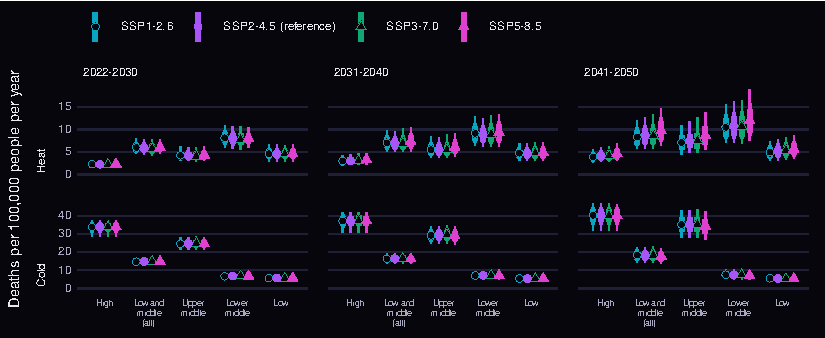
\includegraphics[width=0.9\textwidth,height=0.72\textheight,keepaspectratio]{figures-2026-11-18/fig_income_rates.pdf}

  \footnotesize\raggedright
  Official classification file (October 2026), now with low and middle income combined. Cook Islands, Niue and Tokelau are now high income (territories of New Zealand). Crude rates: age structure explains 64 to 71\% of the heat-rate gap between low and lower-middle income, and more than all of the cold gap.
\end{frame}

\end{document}
